\documentclass[portuguese]{sbc2025}%

%\usepackage{graphicx}% já está incluido na classe
%\usepackage[utf8]{inputenc} % obsoleto, desnecessário

\usepackage[misc,geometry]{ifsym} 

%%%%  %\usepackage{fontspec}

%% Os problemas com a classe eram originados por carregarem ambos os
%% pacotes fontenc e fontspec simultaneamente. Agora a classe detecta
%% qual engine está em uso e se for o pdflates então carrega o
%% fontenc. Se forem o xelatex ou lualatex então carrega o
%% fontspec. Eu particularemnte prefiro o lualatex ou o xetex


% \usepackage{fontawesome} %%% incluido na classe. Desnecessário
% chamá-lo aqui


%%%% \usepackage{academicons}
%%%% outro encrenqueiro que se tornou desnecessario. Deste typeface só
%%%% se usava o glifo do orcid e o codigo interno bombava.
%%%% Substitui pelo pacote orcidlink (carregado internamete na classe)
%%%% e consertei o codigo na classe.


%\usepackage{color} % carregada dentro da classe
%\usepackage{hyperref} % carregada dentro da classe

\usepackage{aas_macros}
\usepackage[bottom]{footmisc}

%\usepackage{supertabular}
%\usepackage{multicol}
%\usepackage{multirow}
%% O pacote tabularray é muito melhor para
% a criacao de tabela complexas e/ou loooongas; tudo de modo simples.
%% Torna o uso de multicol e multirow desnecessarios

\usepackage{tabularray}


\usepackage{afterpage}
\usepackage{url}
\usepackage{pifont}


\setcitestyle{square}


\definecolor{engtitle}{rgb}{0.5,0.5,0.5}
\definecolor{orcidlogo}{rgb}{0.37,0.48,0.13}
\definecolor{unilogo}{rgb}{0.16, 0.26, 0.58}
\definecolor{maillogo}{rgb}{0.58, 0.16, 0.26}
\definecolor{darkblue}{rgb}{0.0,0.0,0.0}
\hypersetup{colorlinks,breaklinks,
            linkcolor=darkblue,urlcolor=darkblue,
            anchorcolor=darkblue,citecolor=darkblue}
%\hypersetup{colorlinks,citecolor=blue,linkcolor=blue,urlcolor=blue}

%%%%%%% IMPORTANT: We disable hyperlinks by default with this line, to avoid the error "\pdfendlink ended up in different nesting level" while writing.
%\hypersetup{draft}



\begin{document}

\jid{REIC}
\jtitle{Revista Eletrônica de Iniciação Científica em Computação, 2025, XX:1}
\issn{1519-8219}
\doi{10.5753/reic.2025.XXXXXX}
\copyrightstatement{This work is licensed under a Creative Commons Attribution 4.0 International License}
\jyear{2025}

\category{Artigo de Pesquisa}
\title[O Computador Sempre Erra: Uma Exploração Gráfica dos Efeitos da Aritmética de Ponto Flutuante]{O Computador Sempre Erra: Uma Exploração Gráfica dos Efeitos da Aritmética de Ponto Flutuante}
\engtitle{\textcolor{engtitle}{The Computer Always Errs: A Graphical Exploration of Floating-Point Arithmetic Effects}}

%THE ORCID IS MANDATORY FOR EACH AUTHOR IN JBCS
\author[Ribas et al. 2025]{
\affil{\textbf{Enzo Rocha L. Diniz Ribas}~\orcidlink{0009-0002-4136-2182}~\textcolor{blue}{\faEnvelopeO}~~[{Centro Federal de Educação Tecnológica de Minas Gerais}~|\href{mailto:enzorochaleitedinizribas@gmail.com}{~{enzorochaleitedinizribas@gmail.com}}~]}

\affil{\textbf{Daniel Paz }~\orcidlink{0000-0000-0000-0000}~~[{Centro Federal de Educação Tecnológica de Minas Gerais}~|\href{mailto:danieldspazini3@gmail.com}{{\textit{danieldspazini3@gmail.com}}}~]}

% \affil{\textbf{Enzo Rocha L. Diniz Ribas}~\orcidlink{0009-0002-4136-2182}~\textcolor{blue}{\faEnvelopeO}~~[{Centro Universitário Dom Helder Câmara}~|\href{mailto:enzorochaleitedinizribas@gmail.com}{~{\textit{enzorochaleitedinizribas@gmail.com}}}~]}

% \affil{\textbf{Enzo Rocha L. Diniz Ribas}~\orcidlink{0009-0002-4136-2182}~\textcolor{blue}{\faEnvelopeO}~~[{Centro Universitário Dom Helder Câmara}~|\href{mailto:enzorochaleitedinizribas@gmail.com}{~{\textit{enzorochaleitedinizribas@gmail.com}}}~]}

}

%\begin{license}
%Published under the Creative Commons Attribution 4.0 International Public License (CC BY 4.0)
%\end{license}

\begin{frontmatter}

\maketitle

\begin{mail}
Centro Federal de Educação Tecnológica de Minas Gerais,  Av. Amazonas, 7675 - Nova Gameleira, Belo Horizonte - MG, 30510-000. 
\end{mail}

\begin{abstract-pt}
  PREVISAO: 500 a 750 palavras
  Este artigo tem como objetivo analisar quais são as principais vantagens e desvantagens de diversas bibliotecas e linguagens de programação utilizadas para visão computacional. A análise é feita com base em critérios como facilidade de uso, curva de aprendizado, comunidade de suporte, compatibilidade com diferentes plataformas, etc.. O estudo inclui uma revisão geral das principais bibliotecas e linguagens mais populares, como OpenCV, TensorFlow, YOLO, JavaCV, VisionWorks, BoofCV, OpenIMAJ, Halcon, SimpleCV entre outras, destacando suas características específicas e casos de uso ideais. Além disso, são apresentados exemplos práticos de aplicação dessas ferramentas em projetos reais, ilustrando como cada uma pode ser utilizada para resolver problemas comuns em visão computacional. A conclusão do artigo oferece recomendações para desenvolvedores e pesquisadores sobre a escolha da biblioteca ou linguagem mais adequada para suas necessidades específicas.
\end{abstract-pt}

\begin{abstract-en}
This text, formatted as a scientific article, aims to present the new SBC paper template, describing its main features and explaining how it should be used. This version, more specifically, should be used exclusively for articles written in Portuguese that will be published in any event proceeding series at SBC OpenLib. The abstract in Portuguese, as you can see in this example, must be before the abstract in English and must have between 500 and 750 words.
\end{abstract-en}

\begin{pchaves}
Mathematical Modeling, Scientific Computing, Numerical Analysis, Floating-Point Arithmetic, Last Place Units, Computational Math
\end{pchaves}

\begin{keywords}
Mathematical Modeling, Scientific Computing, Numerical Analysis, Floating-Point Arithmetic, Last Place Units, Computational Math
\end{keywords}

\begin{dates}
% This information will be provided by the editor before publishing the paper
\noindent{\sffamily\textbf{Recebido/Received:}} DD Month YYYY~~~$\bullet$~~~
{\sffamily\textbf{Aceito/Accepted:}} DD Month YYYY~~~$\bullet$~~~
{\sffamily\textbf{Publicado/Published:}} DD Month YYYY
\end{dates}


%\begin{license}
%Published under the Creative Commons Attribution 4.0 International Public License (CC BY 4.0)
%\end{license}

\end{frontmatter}
 

\section{Introdução}
\label{sec:intro}

Observações iniciais do Prof. Ralha:
\begin{itemize}
    \item Este arquivo faz uso ``implícito"\ de texto em latim que é provido por um certo pacote---não vou citar o nome---que desenvolvedores de classes \LaTeX\ usam para facilitar testes. Vi que esse pacote não está incluido no preâmbulo deste documento. Ainda bem!
    \item por gentileza, entendam que publicar em jornais científicos está relacionado a tipografia profissional. Então deixem este aspecto para o \LaTeX. Seria aconselhável a leitura de textos em typografia para que entendam que ``editoração de textos'' feita por produtos comerciais tipo eh ... vocês sabem quais! não é nem de perto algo que se aproxime da tipografia!
    \item Por óbvio, deve-se sempre iniciar a criação de um arquivo \TeX\ pelo seu preâmbulo. Deve-se evitar \textit{tomar emprestado} templates de outras pessoas. Tenho observado que muitos ``usuários'' não observam este fato levando a casos em que o arquivo inclui o mesmo pacote duas, três e até quatro vezes.
\end{itemize}

A classe \textsl{sbc2025} é projetada para trabalhar com os \textit{engines} pdftex e luatex. Dessa forma, deve-se compilar o documento 
\begin{enumerate}
    \item no Overleaf, ajustando no menu opção de compilação para \textbf{xelatex} ou \textbf{lualatex}.\footnote{Os engines são denominados xetex e luatex. Já os comandos de compilação são \textsl{xelatex} e \textsl{lualatex}.}
    \item se compilando localmente, na sua IDE faça o ajuste do compilador. Se usuário raiz, no terminal de comando, digite \textsl{xelatex filename} ou \textsl{lualatex filename}. Não é necessário digitar a extensão \textsl{tex}.
\end{enumerate}

A classe \textsl{sbc2025} inclui internamente os seguintes pacotes:
\begin{itemize}
    \item xcolor
    \item graphicx
    \item amsmath amssymb
    \item hyperref
    \item babel
\end{itemize}
\noindent consequentemente, não há necessidade de incluí-los no preâmbulo.

{\bfseries Quem tentar compilar usando a opção \texttt{pdflatex} no Overleaf vai receber uma mensagem de erro solicitando o usuário a ajustar a opção de compilação.}

Para a pergunta \textit{Por que não funciona com o \texttt{pdflatex}}?  A resposta é: \textbf{fontes!} Pdflatex usa um esquema de codificação de fontes complexo. 
O fonte \texttt{academicons}\footnote{Do fonte em questão usa-se apenas o glifo associado ao Orchid.} não tem as definições necessárias para uso com o \texttt{pdflatex}. Enquanto isso não for realizado, \texttt{pdflatex} não pode ser usado. 



\section{Revisão Bibliográfica}

A revisão bibliográfica permitiu identificar as principais bibliotecas e linguagens de programação utilizadas em visão computacional, bem como suas características, vantagens e desvantagens. A seguir, são apresentadas as principais ferramentas analisadas:

\subsection{Visão computacional}
Visão computacional é o campo de estudo que busca permitir aos computadores descrever e interpretar o mundo físico. Ela envolve o desenvolvimento de algoritmos e técnicas de processamento, análise e extração de informações de imagens e vídeos. A visão computacional é amplamente utilizada em diversas aplicações, como reconhecimento facial (autenticação visual), detecção de objetos, análise de imagens médicas, modelagem 3D, entre outras \cite{Szeliski2022}.

\subsection{Linguagens de programação}
Diversas linguagens de programação são utilizadas para desenvolver aplicações de visão computacional. A seguir, são apresentadas algumas características das principais linguagens analisadas:
\begin{itemize}
    \item \textbf{Java}: Java é uma linguagem de programação que se destaca por ser multiplataforma, segura e orientada a objetos. \cite{Schildt2019}. Ela possui pequena gama de bibliotecas e frameworks para visão computacional, como JavaCV, BoofCV e OpenIMAJ, que permitem o desenvolvimento de aplicações nessa área.
    \item \textbf{Python}: Python é uma linguagem de programação gratuita amplamente utilizada em áreas da matemática, ciência de dados, inteligência artificial e visão computacional, devido à sua simplicidade, facilidade de aprendizado e utilização, portabilidade e vasta quantidade de bibliotecas. \cite{Lutz1999}. Ela possui um ecossistema robusto para processamento de imagens e visão computacional, com bibliotecas como OpenCV, TensorFlow e MediaPipe, que permitem o desenvolvimento de aplicações complexas de forma acessível e eficiente.
    \item \textbf{C}: 
    % C é uma linguagem de programação de baixo nível que oferece controle preciso sobre os recursos do sistema. Ela é amplamente utilizada em aplicações de visão computacional que exigem alto desempenho e eficiência, como processamento de imagens em tempo real e sistemas embarcados.
    \item \textbf{C++}: 
    % C++ é uma linguagem de programação de alto desempenho que é amplamente utilizada em aplicações de visão computacional que exigem processamento em tempo real. Ela oferece controle preciso sobre os recursos do sistema e é frequentemente utilizada em conjunto com bibliotecas como OpenCV para desenvolvimento de algoritmos de visão computacional.
\end{itemize}

\subsection{Bibliotecas de visão computacional}
Diversas bibliotecas e linguagens de programação são utilizadas para desenvolver aplicações de visão computacional. A seguir, são apresentadas algumas das principais ferramentas analisadas:
\begin{itemize}
    \item \textbf{OpenCV}:
    \item \textbf{TensorFlow}: 
    \item \textbf{YOLO (You Only Look Once)}: 
    \item \textbf{JavaCV}: 
    \item \textbf{VisionWorks}: 
    \item \textbf{BoofCV}: 
    \item \textbf{OpenIMAJ}: 
    \item \textbf{Halcon}: 
    \item \textbf{SimpleCV}: 
    
\end{itemize}




\section{Exemplo de Título Nível 1 (Seção)}
Lorem ipsum dolor sit amet, consectetur adipiscing elit, sed do eiusmod tempor incididunt ut labore et dolore magna aliqua. Ut enim ad minim veniam, quis nostrud exercitation ullamco laboris nisi ut aliquip ex ea commodo consequat. Duis aute irure dolor in reprehenderit in voluptate velit esse cillum dolore eu fugiat nulla pariatur. Excepteur sint occaecat cupidatat non proident, sunt in culpa qui officia deserunt mollit anim id est laborum. Lorem ipsum dolor sit amet, consectetur adipiscing elit, sed do eiusmod tempor incididunt ut labore et dolore magna aliqua. Ut enim ad minim veniam, quis nostrud exercitation ullamco laboris nisi ut aliquip ex ea commodo consequat. Duis aute irure dolor in reprehenderit in voluptate velit esse cillum dolore eu fugiat nulla pariatur. Excepteur sint occaecat cupidatat non proident, sunt in culpa qui officia deserunt mollit anim id est laborum.

\subsection{Exemplo de Título Nível 2 (Subseção)}

Lorem ipsum dolor sit amet, consectetur adipiscing elit, sed do eiusmod tempor incididunt ut labore et dolore magna aliqua. Ut enim ad minim veniam, quis nostrud exercitation ullamco laboris nisi ut aliquip ex ea commodo consequat. Duis aute irure dolor in reprehenderit in voluptate velit esse cillum dolore eu fugiat nulla pariatur. Excepteur sint occaecat cupidatat non proident, sunt in culpa qui officia deserunt mollit anim id est laborum.

\begin{quotation}
\textit{This is a longer quotation. Lorem ipsum dolor sit amet, consectetur adipiscing elit, sed do eiusmod tempor incididunt ut labore et dolore magna aliqua. Lorem ipsum dolor sit amet, consectetur adipiscing elit, sed do eiusmod tempor incididunt ut labore et magna aliqua. 
}\end{quotation} 

\subsubsection{Exemplo de Título Nível 3 (Subsubseção)}

Lorem ipsum dolor sit amet, consectetur adipiscing elit, sed do eiusmod tempor incididunt ut labore et dolore magna aliqua. Ut enim ad minim veniam, quis nostrud exercitation ullamco laboris nisi ut aliquip ex ea commodo consequat. Duis aute irure dolor in reprehenderit in voluptate velit esse cillum dolore eu fugiat nulla pariatur. Excepteur sint occaecat cupidatat non proident, sunt in culpa qui officia deserunt mollit anim id est laborum. Lorem ipsum dolor sit amet, consectetur adipiscing elit, sed do eiusmod tempor incididunt ut labore et dolore magna aliqua. Ut enim ad minim veniam, quis nostrud exercitation ullamco laboris nisi ut aliquip ex ea commodo consequat. Duis aute irure dolor in reprehenderit in voluptate velit esse cillum dolore eu fugiat nulla pariatur. Excepteur sint occaecat cupidatat non proident, sunt in culpa qui officia deserunt mollit anim id est laborum.

\paragraph{Exemplo de Título Nível 4 (Parágrafo).}

Lorem ipsum dolor sit amet, consectetur adipiscing elit, sed do eiusmod tempor incididunt ut labore et dolore magna aliqua. Ut enim ad minim veniam, quis nostrud exercitation ullamco laboris nisi ut aliquip ex ea commodo consequat. Duis aute irure dolor in reprehenderit in voluptate velit esse cillum dolore eu fugiat nulla pariatur. Excepteur sint occaecat cupidatat non proident, sunt in culpa qui officia deserunt mollit anim id est laborum. 
Let
\[
x=(x_1,\dots,x_n)\in R^n
\]be an \(n\)-dimensional vector. The sparse PCA problem can be written as
\begin{equation}\label{eq1}
\max\limits_{x}\{x^TAx-\rho\|x\|_0:x^Tx=1\},
\end{equation}
Lorem ipsum dolor sit amet, consectetur adipiscing elit, sed do eiusmod tempor incididunt ut labore et dolore magna aliqua. Ut enim ad minim veniam, quis nostrud exercitation ullamco laboris nisi ut aliquip ex ea commodo consequat. Duis aute irure dolor in reprehenderit in voluptate velit esse cillum dolore eu fugiat nulla pariatur\break equation (\ref{eq1}). 
\[\max\limits_{x}\{x^TAx :x^Tx=1\}.\]
If $A$ Lorem ipsum dolor sit amet, consectetur adipiscing elit, sed do eiusmod tempor incididunt ut labore et dolore magna aliqua. Ut enim ad minim veniam, quis nostrud exercitation ullamco laboris nisi ut aliquip ex ea commodo consequat. 


Equation (\ref{eq1}) is a special case of the following sparse generalized eigenvector problem (GEV):
\begin{equation}\label{GEV}
\max\limits_{x}\{x^TAx-\rho \|x\|_0: x^TBx\leq 1\},
\end{equation}

Lorem ipsum dolor sit amet, consectetur adipiscing elit, sed do eiusmod tempor incididunt ut labore et dolore magna aliqua. Ut enim ad minim veniam, quis nostrud exercitation ullamco laboris nisi ut aliquip ex ea commodo consequat. Duis aute irure dolor in reprehenderit in voluptate velit esse cillum dolore eu fugiat nulla pariatur. Excepteur sint occaecat cupidatat non proident, sunt in culpa qui officia deserunt mollit anim id est laborum. 

Lorem ipsum dolor sit amet, consectetur adipiscing elit, sed do eiusmod tempor incididunt ut labore et dolore magna aliqua. Ut enim ad minim veniam, quis nostrud exercitation ullamco laboris nisi ut aliquip ex ea commodo consequat. Duis aute irure dolor in reprehenderit in voluptate velit esse cillum dolore eu fugiat nulla pariatur. Excepteur sint occaecat cupidatat non proident, sunt in culpa qui officia deserunt mollit anim id est laborum \textbf{Table~\ref{tab2}}.



\section{Exemplo de Título Nível 1}

Lorem ipsum dolor sit amet, consectetur adipiscing elit, sed do eiusmod tempor incididunt ut labore et dolore magna aliqua. Ut enim ad minim veniam, quis nostrud exercitation ullamco laboris nisi ut aliquip ex ea commodo consequat. Duis aute irure dolor in reprehenderit in voluptate velit esse cillum dolore eu fugiat nulla pariatur. Excepteur sint occaecat cupidatat non proident, sunt in culpa qui officia deserunt mollit anim id est laborum. Lorem ipsum dolor sit amet, consectetur adipiscing elit, sed do eiusmod tempor incididunt ut labore et dolore magna aliqua. Ut enim ad minim veniam, quis nostrud exercitation ullamco laboris nisi ut aliquip ex ea commodo consequat. Duis aute irure dolor in reprehenderit in voluptate velit esse cillum dolore eu fugiat nulla pariatur. Excepteur sint occaecat cupidatat non proident, sunt in culpa qui officia deserunt mollit anim id est laborum.


\begin{table*}
\caption{Exemplo de legenda de tabela.  Duis aute irure dolor in reprehenderit in voluptate velit esse cillum dolore eu fugiat nulla pariatur. Excepteur sint occaecat cupidatat non proident, sunt in culpa qui officia deserunt mollit.} 
\centering
\begin{tabular*}{\textwidth}{@{}c\x c\x c\x c\x c\x c\x c\x c\x c\x c\x c\x c@{}}
\hline \hline
 Número   &  Vel (km/h)   & $\alpha$ (m/s$^2$)    &  $\epsilon^{(1)}$  &  $\epsilon^{(2)}$ 
         & $\delta^{(1)}$ & $\delta^{(2)}$  &  $\delta^{(3)}$    & $\gamma^{(1)}$ 
         & $\gamma^{(2)}$ & $\alpha^{(1)}$  & $\alpha^{(2)}$ \\
%
\hline
 1 & 3.5 & 2.0 & 0.20 & -0.05 & 0.00 & -0.20 & -0.05 & 0.20 & ~0.05 & 20 & 10 \\ 
 2 & 2.5 & 1.5 & 0.10 & -0.15 & 0.05 & -0.15 & ~0.00 & 0.10 & -0.05 & 20 & 40 \\ 
 3 & 3.0 & 1.8 & 0.20 & -0.05 & 0.25 & ~0.05 & ~0.20 & 0.15 & ~0.00 & 20 & 70$^a$ \\
\hline \hline
\end{tabular*}\label{tab2}
\end{table*}

Lorem ipsum dolor sit amet, consectetur adipiscing elit, sed do eiusmod tempor incididunt ut labore et dolore magna aliqua. Ut enim ad minim veniam, quis nostrud exercitation ullamco laboris nisi ut aliquip ex ea commodo consequat. Duis aute irure dolor in reprehenderit in voluptate velit esse cillum dolore eu fugiat nulla pariatur. Excepteur sint occaecat cupidatat non proident, sunt in culpa qui officia deserunt mollit anim id est laborum. Lorem ipsum dolor sit amet, consectetur adipiscing elit, sed do eiusmod tempor incididunt ut labore et dolore magna aliqua. Ut enim ad minim veniam, quis nostrud exercitation ullamco laboris nisi ut aliquip ex ea commodo consequat. Duis aute irure dolor in reprehenderit in voluptate velit esse cillum dolore eu fugiat nulla pariatur. Excepteur sint occaecat cupidatat non proident, sunt in culpa qui officia deserunt mollit anim id est laborum.

\begin{itemize}
\item Esse é um exemplo de lista de tópicos. Lorem ipsum dolor sit amet, consectetur adipiscing elit, sed do eiusmod tempor incididunt.
\item Lorem ipsum dolor sit amet, consectetur adipiscing elit, sed do eiusmod tempor incididunt ut labore et dolore magna aliqua. Ut enim ad minim veniam.
\item Lorem ipsum dolor sit amet, consectetur adipiscing elit, sed do eiusmod tempor incididunt ut labore et dolore magna aliqua. Ut enim ad minim veniam.
\end{itemize}

Lorem ipsum dolor sit amet, consectetur adipiscing elit, sed do eiusmod tempor incididunt ut labore et dolore magna aliqua. Ut enim ad minim veniam, quis nostrud exercitation ullamco laboris nisi ut aliquip ex ea commodo consequat. Duis aute irure dolor in reprehenderit in voluptate velit esse cillum dolore eu fugiat nulla pariatur. Excepteur sint occaecat cupidatat non proident, sunt in culpa qui officia deserunt mollit anim id est laborum. Lorem ipsum dolor sit amet, consectetur adipiscing elit, sed do eiusmod tempor incididunt ut labore et dolore magna aliqua. Ut enim ad minim veniam, quis nostrud exercitation ullamco laboris nisi ut aliquip ex ea commodo consequat. Duis aute irure dolor in reprehenderit in voluptate velit esse cillum dolore eu fugiat nulla pariatur. Excepteur sint occaecat cupidatat non proident, sunt in culpa qui officia deserunt mollit anim id est laborum.

\begin{enumerate}%
\item Esse é um exemplo de lista numerada. Lorem ipsum dolor sit amet, consectetur adipiscing elit, sed do eiusmod tempor incididunt.
\item Lorem ipsum dolor sit amet, consectetur adipiscing elit, sed do eiusmod tempor incididunt ut labore et dolore magna aliqua. Ut enim ad minim veniam.
\item Lorem ipsum dolor sit amet, consectetur adipiscing elit, sed do eiusmod tempor incididunt ut labore et dolore magna aliqua. Ut enim ad minim veniam.
\end{enumerate}

Lorem ipsum dolor sit amet, consectetur adipiscing elit, sed do eiusmod tempor incididunt ut labore et dolore magna aliqua. Ut enim ad minim veniam, quis nostrud exercitation ullamco laboris nisi ut aliquip ex ea commodo consequat. Duis aute irure dolor in reprehenderit in voluptate velit esse cillum dolore eu fugiat nulla pariatur. Excepteur sint occaecat cupidatat non proident, sunt in culpa qui officia deserunt mollit anim id est laborum. Lorem ipsum dolor sit amet, consectetur adipiscing elit, sed do eiusmod tempor incididunt ut labore et dolore magna aliqua. Ut enim ad minim veniam, quis nostrud exercitation ullamco laboris nisi ut aliquip ex ea commodo consequat. Duis aute irure dolor in reprehenderit in voluptate velit esse cillum dolore eu fugiat nulla pariatur. Excepteur sint occaecat cupidatat non proident, sunt in culpa qui officia deserunt mollit anim id est laborum.

Lorem ipsum dolor sit amet, consectetur adipiscing elit, sed do eiusmod tempor incididunt ut labore et dolore magna aliqua. Ut enim ad minim veniam, quis nostrud exercitation ullamco laboris nisi ut aliquip ex ea commodo consequat. Duis aute irure dolor in reprehenderit in voluptate velit esse cillum dolore eu fugiat nulla pariatur. Excepteur sint occaecat cupidatat non proident, sunt in culpa qui officia deserunt mollit anim id est laborum. Lorem ipsum dolor sit amet, consectetur adipiscing elit, sed do eiusmod tempor incididunt ut labore et dolore magna aliqua. Ut enim ad minim veniam, quis nostrud exercitation ullamco laboris nisi ut aliquip ex ea commodo consequat. Duis aute irure dolor in reprehenderit in voluptate velit esse cillum dolore eu fugiat nulla pariatur. Excepteur sint occaecat cupidatat non proident, sunt in culpa qui officia deserunt mollit anim id est laborum.


\subsection{Exemplo de Título Nível 2}

Lorem ipsum dolor sit amet, consectetur adipiscing elit, sed do eiusmod tempor incididunt ut labore et dolore magna aliqua. Ut enim ad minim veniam, quis nostrud exercitation ullamco laboris nisi ut aliquip ex ea commodo consequat. Duis aute irure dolor in reprehenderit in voluptate velit esse cillum dolore eu fugiat nulla pariatur. Excepteur sint occaecat cupidatat non proident, sunt in culpa qui officia deserunt mollit anim id est laborum. Lorem ipsum dolor sit amet, consectetur adipiscing elit, sed do eiusmod tempor incididunt ut labore et dolore magna aliqua. Ut enim ad minim veniam, quis nostrud exercitation ullamco laboris nisi ut aliquip ex ea commodo consequat. Duis aute irure dolor in reprehenderit in voluptate velit esse cillum dolore eu fugiat nulla pariatur. Excepteur sint occaecat cupidatat non proident, sunt in culpa qui officia deserunt mollit anim id est laborum \textbf{Figure \ref{Fig1}}.

Lorem ipsum dolor sit amet, consectetur adipiscing elit, sed do eiusmod tempor incididunt ut labore et dolore magna aliqua. Ut enim ad minim veniam, quis nostrud exercitation ullamco laboris nisi ut aliquip ex ea commodo consequat. Duis aute irure dolor in reprehenderit in voluptate velit esse cillum dolore eu fugiat nulla pariatur. Excepteur sint occaecat cupidatat non proident, sunt in culpa qui officia deserunt mollit anim id est laborum. Lorem ipsum dolor sit amet, consectetur adipiscing elit, sed do eiusmod tempor incididunt ut labore et dolore magna aliqua. Ut enim ad minim veniam, quis nostrud exercitation ullamco laboris nisi ut aliquip ex ea commodo consequat. Duis aute irure dolor in reprehenderit in voluptate velit esse cillum dolore eu fugiat nulla pariatur. Excepteur sint occaecat cupidatat non proident, sunt in culpa qui officia deserunt mollit anim id est laborum.

Lorem ipsum dolor sit amet, consectetur adipiscing elit, sed do eiusmod tempor incididunt ut labore et dolore magna aliqua. Ut enim ad minim veniam, quis nostrud exercitation ullamco laboris nisi ut aliquip ex ea commodo consequat. Duis aute irure dolor in reprehenderit in voluptate velit esse cillum dolore eu fugiat nulla pariatur. Excepteur sint occaecat cupidatat non proident, sunt in culpa qui officia deserunt mollit anim id est laborum. Lorem ipsum dolor sit amet, consectetur adipiscing elit, sed do eiusmod tempor incididunt ut labore et dolore magna aliqua. Ut enim ad minim veniam, quis nostrud exercitation ullamco laboris nisi ut aliquip ex ea commodo consequat. Duis aute irure dolor in reprehenderit in voluptate velit esse cillum dolore eu fugiat nulla pariatur. Excepteur sint occaecat cupidatat non proident, sunt in culpa qui officia deserunt mollit anim id est laborum.

\begin{figure}
\begin{center}
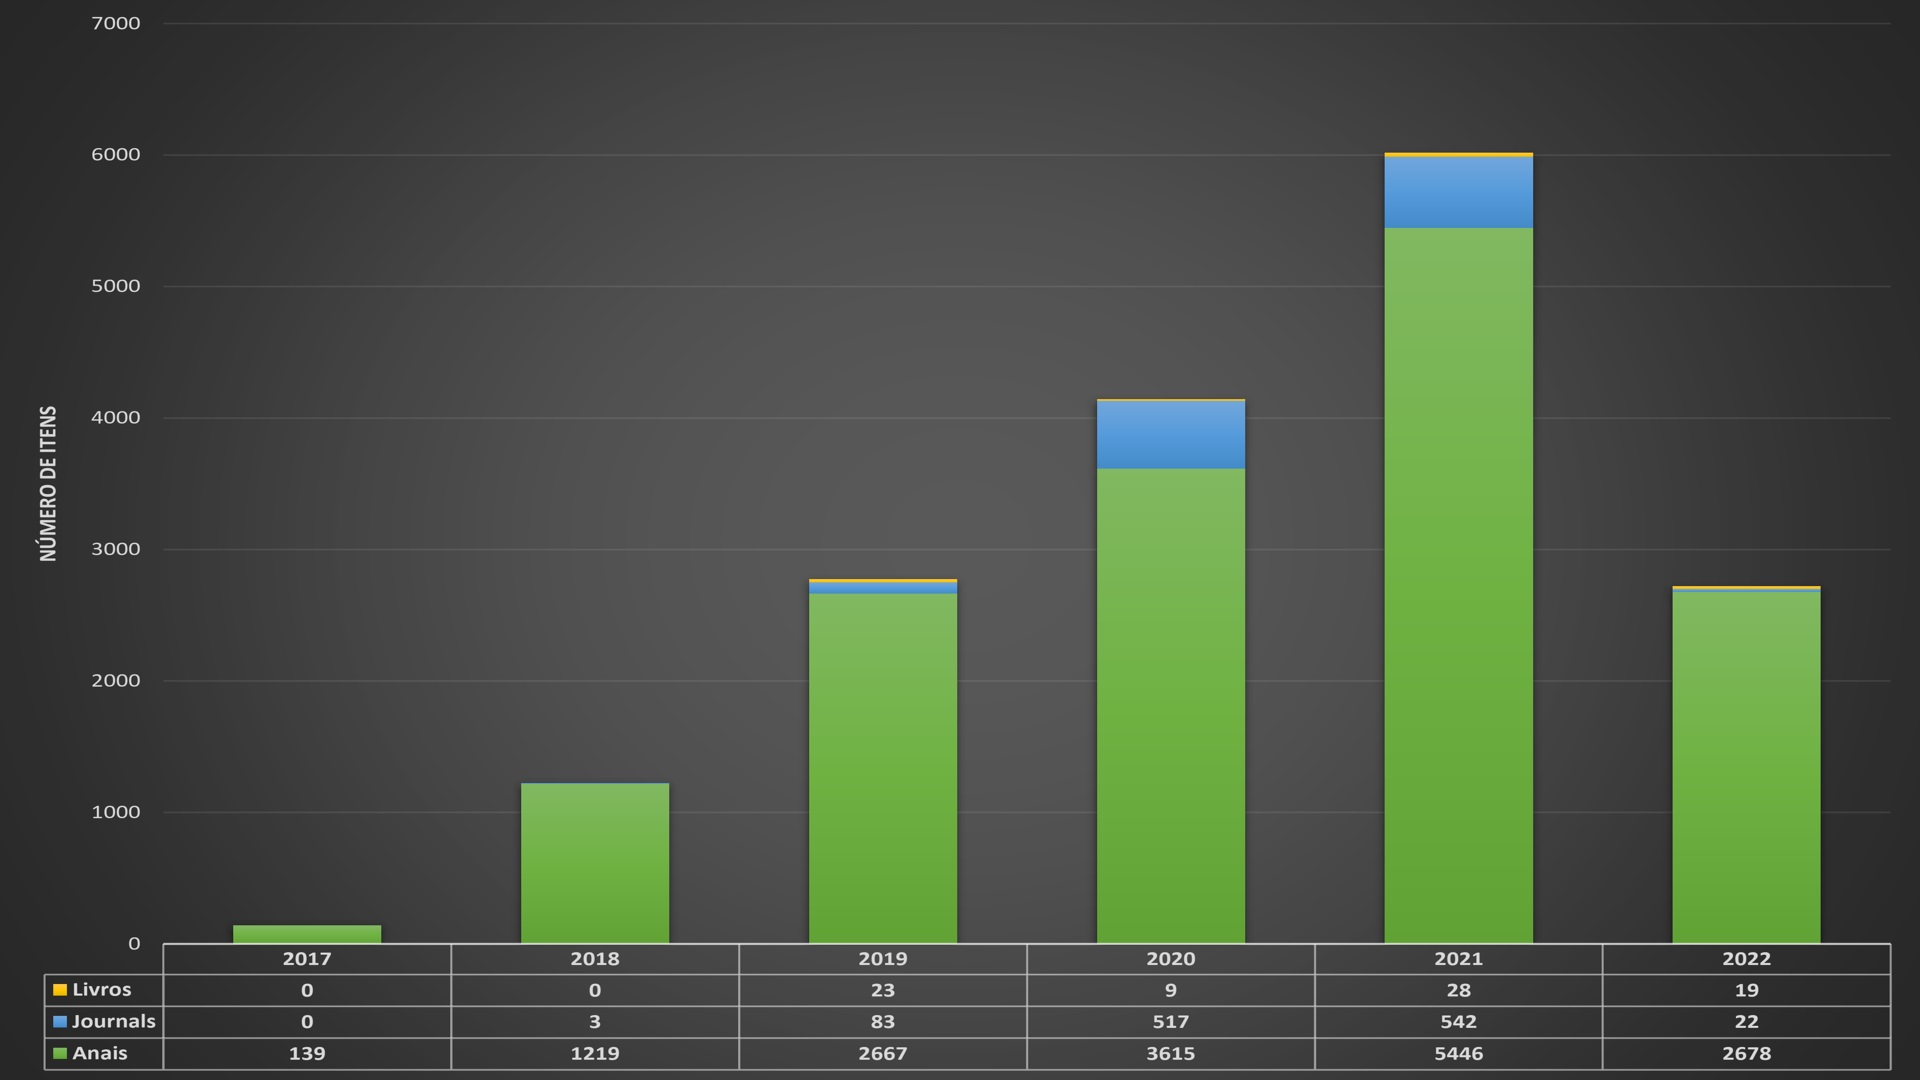
\includegraphics[width=\columnwidth]{sol.jpg}
\caption{Exemplo de legenda de figura.}\label{Fig1}
\end{center}
\end{figure}

Lorem ipsum dolor sit amet, consectetur adipiscing elit, sed do eiusmod tempor incididunt ut labore et dolore magna aliqua. Ut enim ad minim veniam, quis nostrud exercitation ullamco laboris nisi ut aliquip ex ea commodo consequat. Duis aute irure dolor in reprehenderit in voluptate velit esse cillum dolore eu fugiat nulla pariatur. Excepteur sint occaecat cupidatat non proident, sunt in culpa qui officia deserunt mollit anim id est laborum. Lorem ipsum dolor sit amet, consectetur adipiscing elit, sed do eiusmod tempor incididunt ut labore et dolore magna aliqua. Ut enim ad minim veniam, quis nostrud exercitation ullamco laboris nisi ut aliquip ex ea commodo consequat. Duis aute irure dolor in reprehenderit in voluptate velit esse cillum dolore eu fugiat nulla pariatur. Excepteur sint occaecat cupidatat non proident, sunt in culpa qui officia deserunt mollit anim id est laborum.

Lorem ipsum dolor sit amet, consectetur adipiscing elit, sed do eiusmod tempor incididunt ut labore et dolore magna aliqua. Ut enim ad minim veniam, quis nostrud exercitation ullamco laboris nisi ut aliquip ex ea commodo consequat. Duis aute irure dolor in reprehenderit in voluptate velit esse cillum dolore eu fugiat nulla pariatur. Excepteur sint occaecat cupidatat non proident, sunt in culpa qui officia deserunt mollit anim id est laborum. Lorem ipsum dolor sit amet, consectetur adipiscing elit, sed do eiusmod tempor incididunt ut labore et dolore magna aliqua. Ut enim ad minim veniam, quis nostrud exercitation ullamco laboris nisi ut aliquip ex ea commodo consequat. Duis aute irure dolor in reprehenderit in voluptate velit esse cillum dolore eu fugiat nulla pariatur. Excepteur sint occaecat cupidatat non proident, sunt in culpa qui officia deserunt mollit anim id est laborum \textbf{Figure \ref{Fig2}}.

\begin{figure*}
\begin{center}
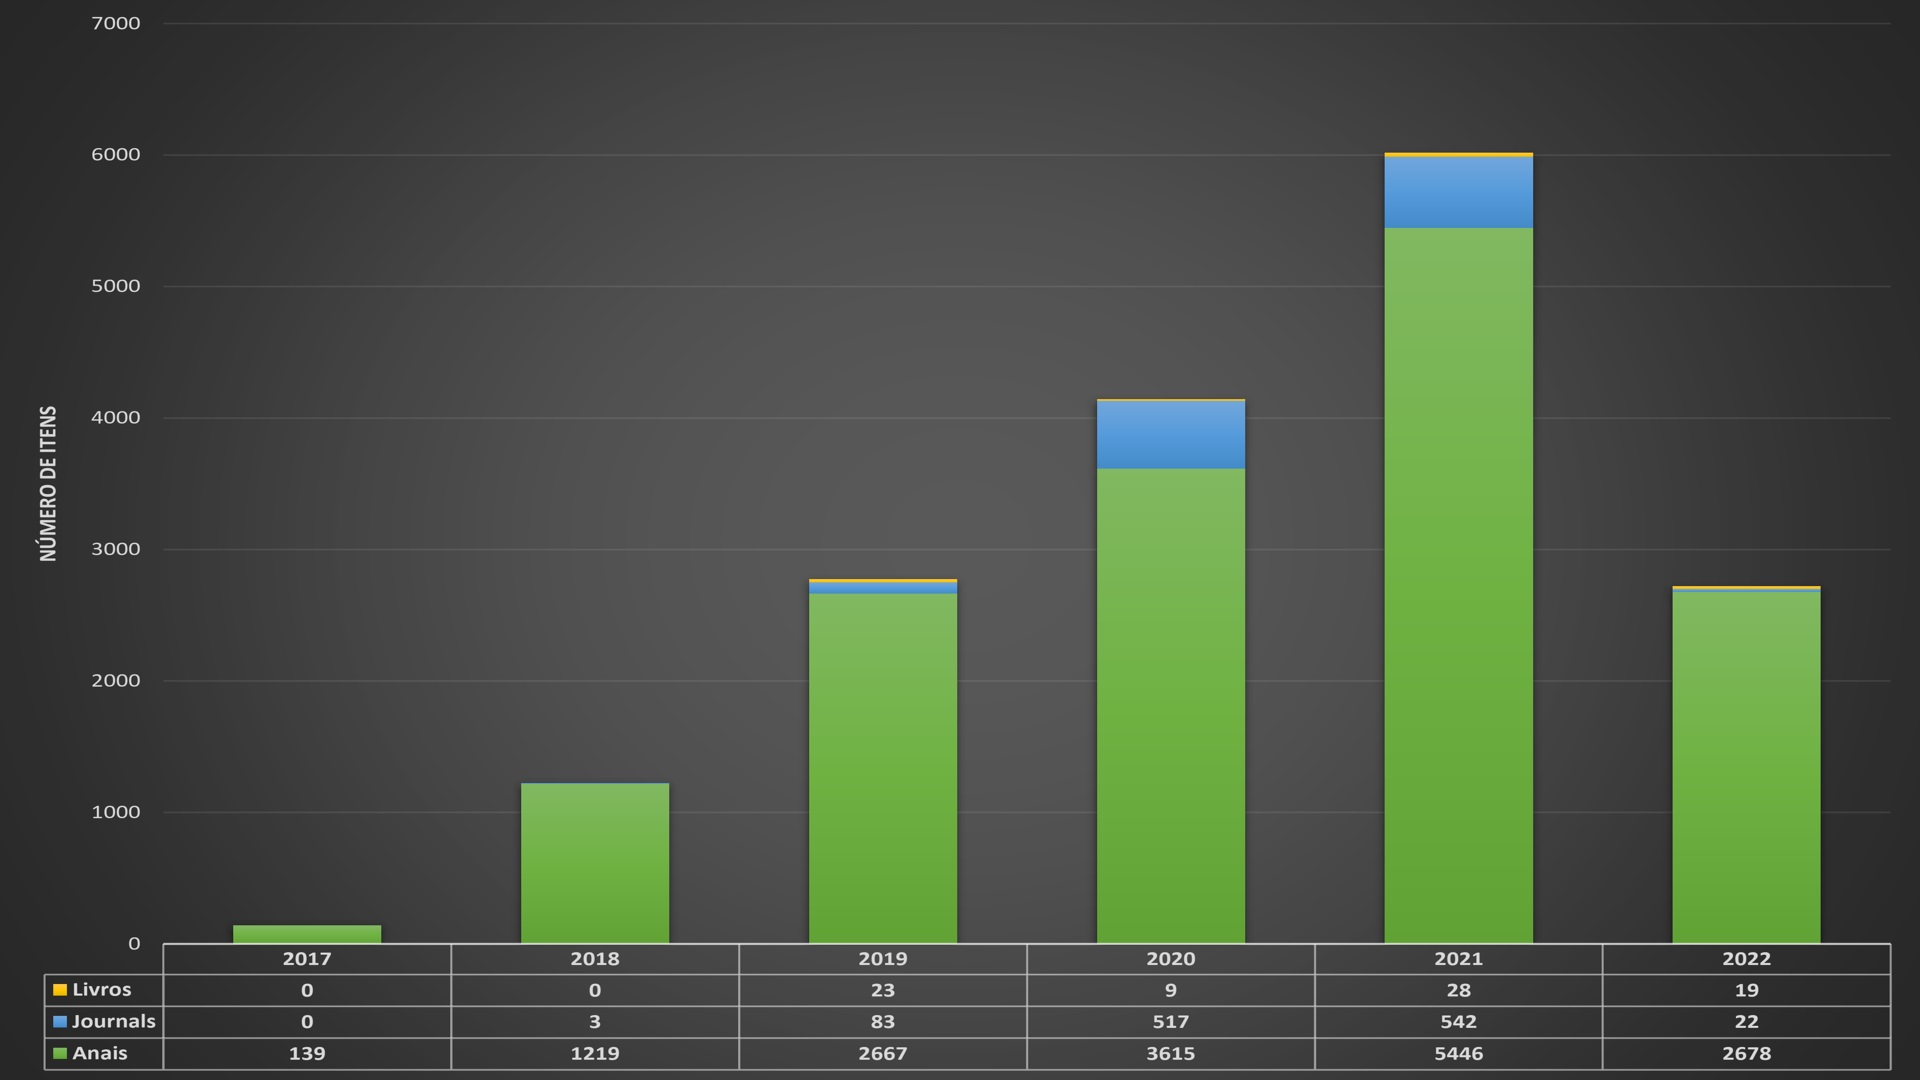
\includegraphics[width=30pc]{sol.jpg}
\caption{{Exemplo de legenda de figura.}}
 \label{Fig2}
\end{center}
\end{figure*}

Lorem ipsum dolor sit amet, consectetur adipiscing elit, sed do eiusmod tempor incididunt ut labore et dolore magna aliqua. Ut enim ad minim veniam, quis nostrud exercitation ullamco laboris nisi ut aliquip ex ea commodo consequat. Duis aute irure dolor in reprehenderit in voluptate velit esse cillum dolore eu fugiat nulla pariatur. Excepteur sint occaecat cupidatat non proident, sunt in culpa qui officia deserunt mollit anim id est laborum. Lorem ipsum dolor sit amet, consectetur adipiscing elit, sed do eiusmod tempor incididunt ut labore et dolore magna aliqua. Ut enim ad minim veniam, quis nostrud exercitation ullamco laboris nisi ut aliquip ex ea commodo consequat. Duis aute irure dolor in reprehenderit in voluptate velit esse cillum dolore eu fugiat nulla pariatur. Excepteur sint occaecat cupidatat non proident, sunt in culpa qui officia deserunt mollit anim id est laborum.

Lorem ipsum dolor sit amet, consectetur adipiscing elit, sed do eiusmod tempor incididunt ut labore et dolore magna aliqua. Ut enim ad minim veniam, quis nostrud exercitation ullamco laboris nisi ut aliquip ex ea commodo consequat. Duis aute irure dolor in reprehenderit in voluptate velit esse cillum dolore eu fugiat nulla pariatur. Excepteur sint occaecat cupidatat non proident, sunt in culpa qui officia deserunt mollit anim id est laborum. Lorem ipsum dolor sit amet, consectetur adipiscing elit, sed do eiusmod tempor incididunt ut labore et dolore magna aliqua. Ut enim ad minim veniam, quis nostrud exercitation ullamco laboris nisi ut aliquip ex ea commodo consequat. Duis aute irure dolor in reprehenderit in voluptate velit esse cillum dolore eu fugiat nulla pariatur. Excepteur sint occaecat cupidatat non proident, sunt in culpa qui officia deserunt mollit anim id est laborum.

Lorem ipsum dolor sit amet, consectetur adipiscing elit, sed do eiusmod tempor incididunt ut labore et dolore magna aliqua. Ut enim ad minim veniam, quis nostrud exercitation ullamco laboris nisi ut aliquip ex ea commodo consequat. Duis aute irure dolor in reprehenderit in voluptate velit esse cillum dolore eu fugiat nulla pariatur. Excepteur sint occaecat cupidatat non proident, sunt in culpa qui officia deserunt mollit anim id est laborum. Lorem ipsum dolor sit amet, consectetur adipiscing elit, sed do eiusmod tempor incididunt ut labore et dolore magna aliqua. Ut enim ad minim veniam, quis nostrud exercitation ullamco laboris nisi ut aliquip ex ea commodo consequat. Duis aute irure dolor in reprehenderit in voluptate velit esse cillum dolore eu fugiat nulla pariatur. Excepteur sint occaecat cupidatat non proident, sunt in culpa qui officia deserunt mollit anim id est laborum.



\paragraph{Exemplo de Título Nível 4.}

Excepteur sint occaecat cupidatat non proident, sunt in culpa qui officia deserunt mollit anim id est laborum. Lorem ipsum dolor sit amet, consectetur adipiscing elit, sed do eiusmod tempor incididunt ut labore et dolore magna aliqua. Ut enim ad minim veniam, quis nostrud exercitation ullamco laboris nisi ut aliquip ex ea commodo consequat. Duis aute irure dolor in reprehenderit in voluptate velit esse cillum dolore eu fugiat nulla pariatur. 

Lorem ipsum dolor sit amet, consectetur adipiscing elit, sed do eiusmod tempor incididunt ut labore et dolore magna aliqua. Ut enim ad minim veniam, quis nostrud exercitation ullamco laboris nisi ut aliquip ex ea commodo consequat. Excepteur sint occaecat cupidatat non proident, sunt in culpa qui officia deserunt mollit anim id est laborum. Lorem ipsum dolor sit amet, consectetur adipiscing elit, sed do eiusmod tempor incididunt ut labore et dolore magna aliqua. Ut enim ad minim veniam, quis nostrud exercitation ullamco laboris nisi ut aliquip ex ea commodo consequat. Duis aute irure dolor in reprehenderit in voluptate velit esse cillum dolore eu fugiat nulla pariatur. Excepteur sint occaecat cupidatat non proident, sunt in culpa qui officia deserunt mollit anim id est laborum.



\section{Conclusão}

Excepteur sint occaecat cupidatat non proident, sunt in culpa qui officia deserunt mollit anim id est laborum. Lorem ipsum dolor sit amet, consectetur adipiscing elit, sed do eiusmod tempor incididunt ut labore et dolore magna aliqua. Ut enim ad minim veniam, quis nostrud exercitation ullamco laboris nisi ut aliquip ex ea commodo consequat. Duis aute irure dolor in reprehenderit in voluptate velit esse cillum dolore eu fugiat nulla pariatur. 

Lorem ipsum dolor sit amet, consectetur adipiscing elit, sed do eiusmod tempor incididunt ut labore et dolore magna aliqua. Ut enim ad minim veniam, quis nostrud exercitation ullamco laboris nisi ut aliquip ex ea commodo consequat. Excepteur sint occaecat cupidatat non proident, sunt in culpa qui officia deserunt mollit anim id est laborum. Lorem ipsum dolor sit amet, consectetur adipiscing elit, sed do eiusmod tempor incididunt ut labore et dolore magna aliqua. Ut enim ad minim veniam, quis nostrud exercitation ullamco laboris nisi ut aliquip ex ea commodo consequat. Duis aute irure dolor in reprehenderit in voluptate velit esse cillum dolore eu fugiat nulla pariatur. Excepteur sint occaecat cupidatat non proident, sunt in culpa qui officia deserunt mollit anim id est laborum \citep{ref5}.



\section{Conclusão}

Excepteur sint occaecat cupidatat non proident, sunt in culpa qui officia deserunt mollit anim id est laborum. Lorem ipsum dolor sit amet, consectetur adipiscing elit, sed do eiusmod tempor incididunt ut labore et dolore magna aliqua. Ut enim ad minim veniam, quis nostrud exercitation ullamco laboris nisi ut aliquip ex ea commodo consequat. Duis aute irure dolor in reprehenderit in voluptate velit esse cillum dolore eu fugiat nulla pariatur. 

Lorem ipsum dolor sit amet, consectetur adipiscing elit, sed do eiusmod tempor incididunt ut labore et dolore magna aliqua. Ut enim ad minim veniam, quis nostrud exercitation ullamco laboris nisi ut aliquip ex ea commodo consequat. Excepteur sint occaecat cupidatat non proident, sunt in culpa qui officia deserunt mollit anim id est laborum. Lorem ipsum dolor sit amet, consectetur adipiscing elit, sed do eiusmod tempor incididunt ut labore et dolore magna aliqua. Ut enim ad minim veniam, quis nostrud exercitation ullamco laboris nisi ut aliquip ex ea commodo consequat. Duis aute irure dolor in reprehenderit in voluptate velit esse cillum dolore eu fugiat nulla pariatur. Excepteur sint occaecat cupidatat non proident, sunt in culpa qui officia deserunt mollit anim id est laborum \citep{ref5}.


\begin{declarations}

\begin{acknowledgements}
ESTA DECLARAÇÃO É OPCIONAL. Este é um texto de agradecimentos com várias linhas. Lorem ipsum dolor sit amet, consectetur adipiscing elit, sed do eiusmod tempor incididunt ut labore et dolore magna aliqua. Ut enim ad minim veniam, quis nostrud exercitation ullamco laboris nisi ut aliquip ex ea commodo consequat.
\end{acknowledgements}

\begin{funding}
ESTA DECLARAÇÃO É OPCIONAL. Esta pesquisa foi financiada por lorem ipsum dolor sit amet, consectetur adipiscing elit.
\end{funding}

\begin{contributions}
ESTA DECLARAÇÃO É OBRIGATÓRIA. Sugerimos que os autores descrevam sua contribuição usando a Taxonomia CRediT (\href{https://credit.niso.org/}{https://credit.niso.org/}) como neste exemplo: JV contribuiu para a concepção deste estudo. CB, RP e CM realizaram os experimentos. JV é o principal contribuidor e escritor deste manuscrito. Todos os autores leram e aprovaram o manuscrito final. 
\end{contributions}

\begin{interests}
ESTA DECLARAÇÃO É OBRIGATÓRIA. Se não houver conflitos de interesse, os autores devem declarar: ``Os autores declaram que não têm nenhum conflito de interesses''. Caso contrário, a declaração deve ser: ``Os autores declaram que têm os seguintes conflito de interesses: lorem ipsum dolor sit amet, consectetur adipiscing elit.''
\end{interests}

\begin{materials}
ESTA DECLARAÇÃO É OBRIGATÓRIA. 
  Se os autores estiverem disponibilizando seus dados e/ou códigos
  abertamente, a declaração deve ser: ``Os conjuntos de dados (e/ou
  softwares) gerados e/ou analisados durante o estudo atual estão
  disponíveis em \ldots''. Caso contrário, a declaração deve ser: ``Os
  conjuntos de dados (e/ou softwares) gerados e/ou analisados durante
  o estudo atual serão feitos mediante solicitação''.
\end{materials}

\begin{furtherinformation}
ESTA DECLARAÇÃO É DESEJÁVEL. Informações adicionais relevantes, como, por exemplo, a aprovação em comitê de ética ou o uso de ferramentas de IA generativa no desenvolvimento do artigo. Essa declaração é opcional, se não houver nada a ser acrescentado, pode ser deixada em branco
\end{furtherinformation}
\end{declarations}



\bibliographystyle{apalike-sol}
\bibliography{refs}

\end{document}
